%!TEX root = ../main.tex

\section{Empirical Analysis}
\label{sec:Analysis}

We first describe six large-scale network datasets.
Then, we describe global network properties,
insights from empirical studies and common assumptions in
network modeling.

\subsection{Datasets}
\label{sec:Datasets}

We consider six citation networks of different scales (size, time) from diverse
sources: research articles, utility patents and judicial cases. ~\Cref{table:datasets} lists their
summary statistics and global network properties.  Three of the six datasets are attributed networks;
that is, each node has a categorical attribute value.

We focus on citation networks for two reasons. First, since nodes in citation networks form
all outgoing edges to existing nodes at the time of joining the network,
these datasets provide a clean basis to study edge formation in
attributed networks. Second, the node-level, temporal information in datasets that span long time periods (e.g. \texttt{USSC})
enables us to study structural properties at different time stages via network snapshots.
Next, we study the structural and attribute properties of these networks.

\subsection{Global Network Properties}
\label{subsec:factors}

Statistical descriptors of network properties ~\cite{newman2010networks}
such as degree distribution, local clustering, and attribute assortativity
quantify the extent to which edge formation shapes global network
structure.

\textbf{Degree distribution:}
Real-world networks tend to exhibit heavy tailed degree distributions in which
a small but significant fraction of the nodes turn into high-degree hubs.
We observe that Log-normal fits, with parameters listed in~\Cref{table:netstats}, well describe
the in-degree distributions, consistent with Broido and
Clauset's~\cite{broido2018scale} observation that scale-free, real-world networks
are rare.

\begin{figure}
 % \vspace{-10pt}
 \centering
 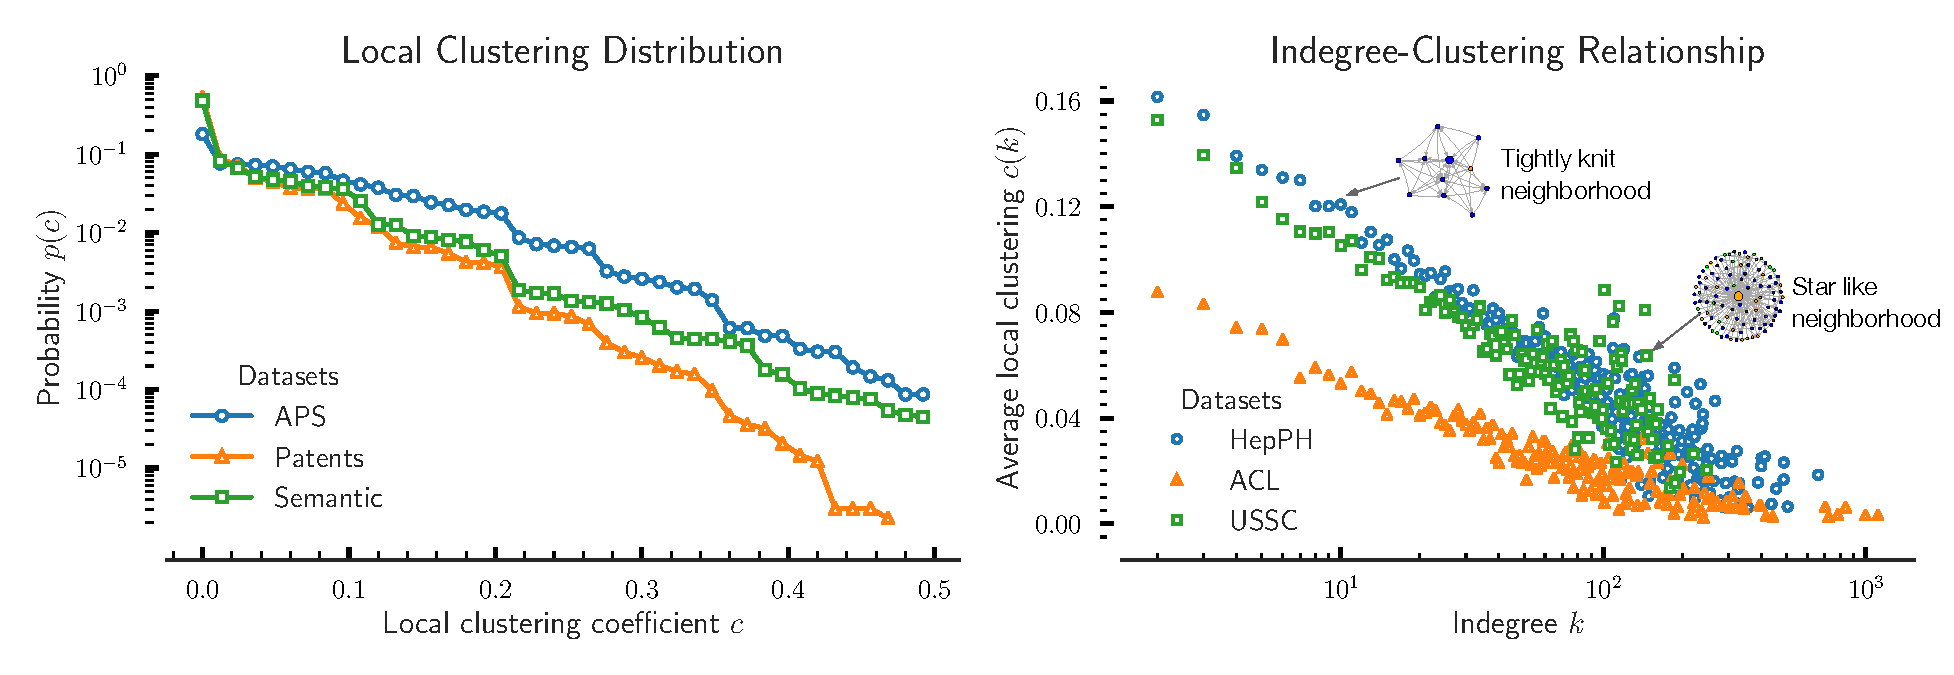
\includegraphics[width=\columnwidth]{clustering}
 \caption{
    Real-world networks exhibit
    skewed local clustering distribution (left subplot) and a negatively correlated
    relationship between in-degree and average local clustering (right subplot).
 }
 \label{fig:cc_dc}
 % \vspace{-10pt}
\end{figure}

\textbf{Local Clustering:}
Real-world networks exhibit high local clustering
(\texttt{LCC}), as shown in~\Cref{table:netstats}. Local
clustering can arise from triadic closure~\cite{simmel1950sociology,
newman2001clustering}, where nodes with common neighbor(s) have an increased
likelihood of forming a connection.
The coefficient of node $i$ equals the probability with which two randomly chosen
neighbors of the node $i$ are connected. In directed networks, the neighborhood
of a node $i$ can refer to the nodes that link to $i$, nodes that
$i$ links to or both. We define the neighborhood to be the set
of all nodes that link to node $i$. In ~\Cref{fig:cc_dc}, we show that (a) average local clustering is not a
representative statistic of the skewed local clustering distributions and (b) real-world networks
exhibit a negative correlation between in-degree and clustering.
That is, low in-degree nodes have small, tightly knit neighborhoods
and high in-degree nodes tend have large, star-shaped neighborhoods.


% Homophily and Assortativity
\textbf{Homophily:}
Attributed networks tend to exhibit homophily~\cite{mcpherson2001birds}, the
phenomenon where similar nodes are more likely to be connected than dissimilar
nodes. The assortativity coefficient ~\cite{newman2002assortative} $r \in [-1,
1]$, quantifies the level of homophily in an attributed network.
Intuitively,
assortativity compares the observed fraction of edges between nodes with the same attribute
value to the expected fraction of edges between nodes with same attribute value
if the edges were rewired randomly. In~\Cref{fig:mixing}, we show that
attributed networks \texttt{ACL}, \texttt{APS} and \texttt{Patents} exhibit
varying level of homophily with assortativity coefficient ranging from $0.07$ to
$0.72$.


\begin{figure}
 \centering
 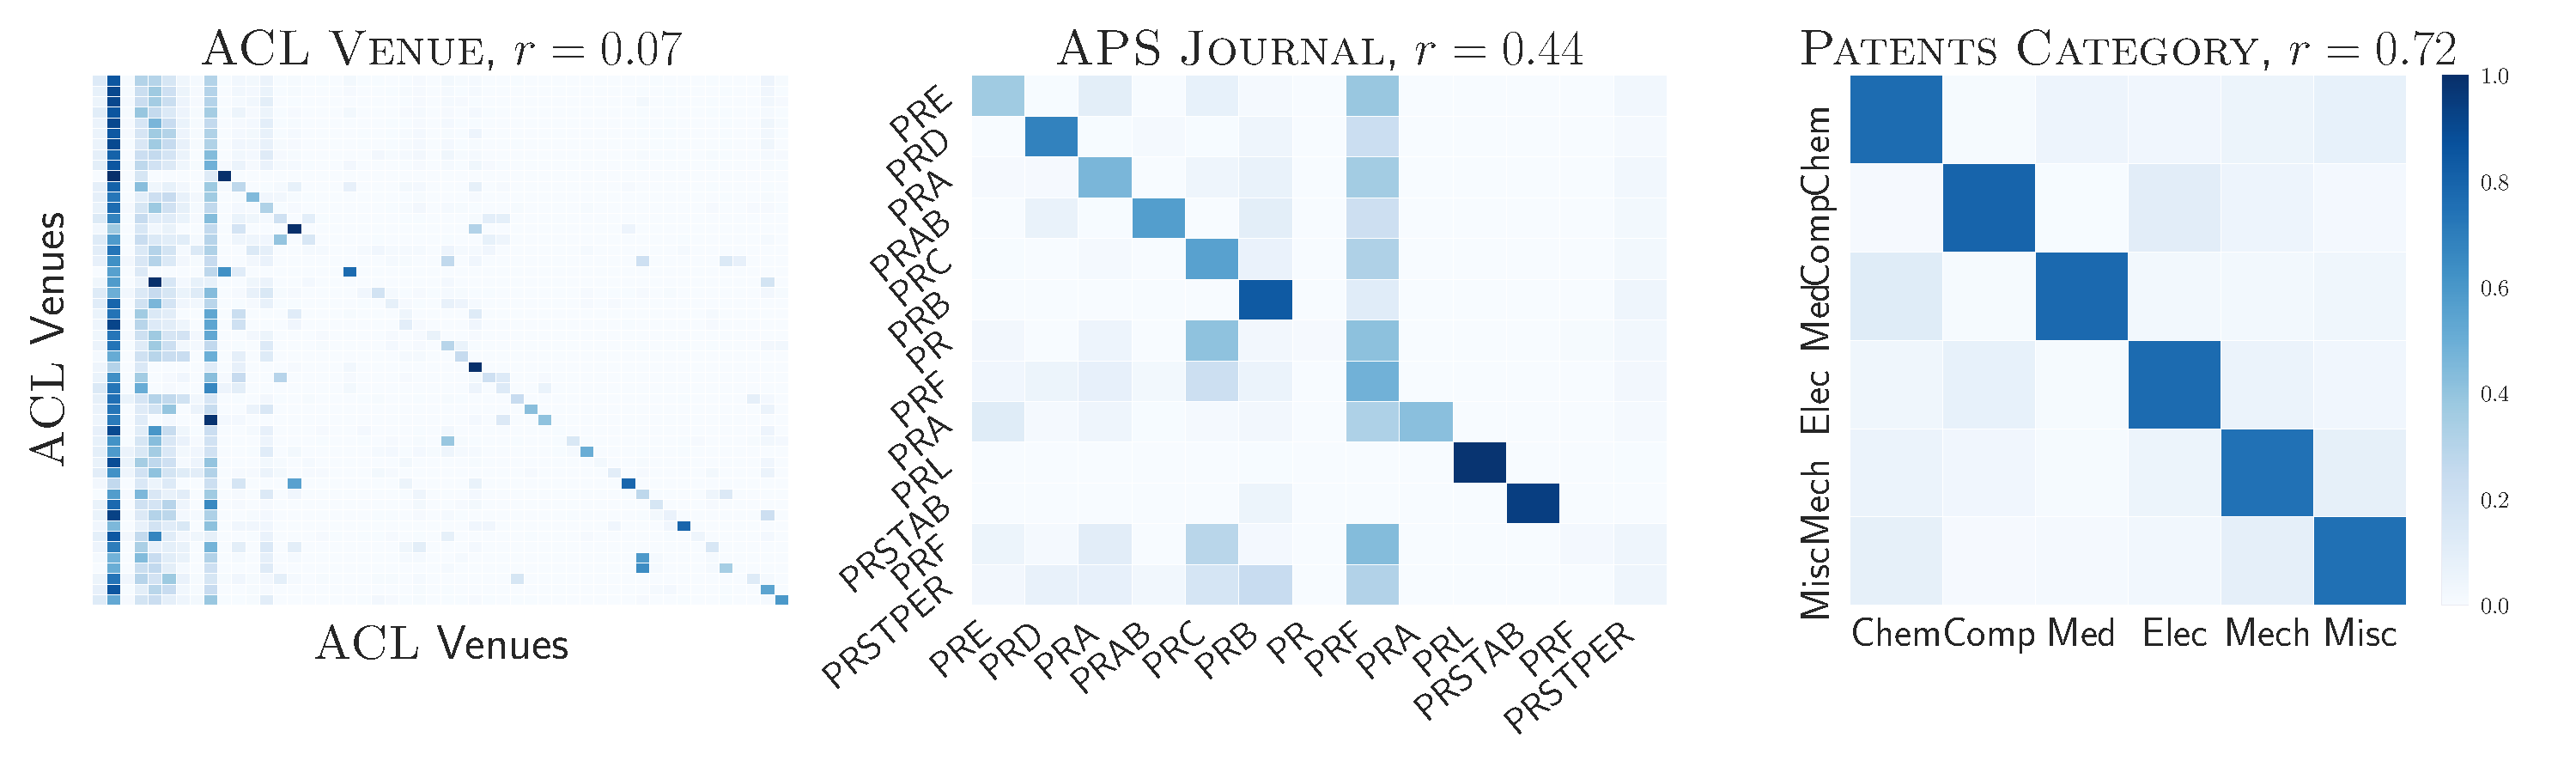
\includegraphics[width=\columnwidth]{homophily}
 \caption{
    Attributed networks \texttt{ACL}, \texttt{APS} and \texttt{Patents} exhibit
    homophily w.r.t attributes \texttt{Venue} ($r=0.07$), \texttt{Journal} ($r=0.44$) and
    \texttt{Category} ($r=0.72$) respectively.
 }
 \label{fig:mixing}
 \vspace{-20pt}
\end{figure}



\textbf{Increasing Out-degree over Time:}
The out-degree of nodes that join real-world networks tends to increase as
functions of network size and time. This phenomenon densifies networks and
can shrink effective diameter over time. Densification tends to exhibit a power law
relationship ~\cite{leskovec2005graphs} between the number of edges $e(t)$ and
nodes $n(t)$ at time $t$: $e(t) \propto n(t)^{\alpha}$.~\Cref{table:netstats}
lists the densification power law (\texttt{DPL}) exponent $\alpha$ of the
network datasets.

To summarize, citation networks tend to be homophilic networks that undergo
accelerated network growth and exhibit regularities in structural properties:
heavy tailed in-degree distribution, skewed local clustering distribution,
negatively correlated degree-clustering relationship, and varying attribute
mixing patterns.

\subsection{Insights from Sociological Studies}

Sociological studies on network formation seek to explain
how individuals form edges in real-world networks.

\textbf{Interplay of Triadic Closure and Homophily:}
Empirical studies~\cite{35626,block2014multidimensional} that analyze the
interplay between triadic closure and homophily
 % in evolving networks
  indicate
that \textit{both} structural proximity and homophily are statistically
significant factors that simultaneously influence edge formation.
Homophilic preferences~\cite{mcpherson2001birds} induce edges between similar
nodes, whereas structural factors such as network distance limit
edge formation to proximate nodes (e.g. friend of a
friend).

\textbf{Bounded Rationality:}
Extensive work~\cite{simon1972theories,gigerenzer1996reasoning,lipman1995information} on
decision making shows that individuals are boundedly rational
actors; constraints such as limited information, cognitive capacity and time impact decision making.
This suggests that resource-constrained individuals that join networks are likely to employ simple rules
to form edges using limited information and partial network access.


Current preferential attachment and fitness-based models
\cite{dorogovtsev2000structure,singh2017relay,barabasi1999emergence}
make two assumptions that are at variance with these findings.
First, by assuming that successive edge formations are independent,
these models disregard the effect of triadic closure and structural proximity.
Second, as discussed in~\cref{sec:Introduction}, these models require complete network
access or knowledge of node-level properties.

Insights from sociological studies indicate that edge formation in real-world
networks comprises biases towards nodes that are similar, well-connected or
structurally proximate. Coupled with empirical analyses, it also motivates
the need to model how resource-constrained edge formation processes collectively
shape global network properties of large-scale networks over time.
